\documentclass[a4paper, 12pt]{article}

\usepackage[UTF8]{ctex}
\usepackage{graphicx}
\usepackage{lipsum}
\usepackage[colorlinks=true]{hyperref}
\usepackage[margin=.5in]{geometry}

\begin{document}
\pagenumbering{gobble}

\large
\title{Web dev}
\author{Joshua Yu}
\date{29 Aug. 2018}
\maketitle
\tableofcontents

%\lipsum[1-5]

\section{Project feature request}
\begin{enumerate}
\item 微信门票列表搜索框,当需要对历史搜索里面的数据进行修改时,点击输入框后文字消失
\end{enumerate}

\section{Things to be done before commit}
\begin{enumerate}

\item Indent using tabs, and set tab size to 2

\item Delete \verb|console.log()|

\item Format document by pressing \verb|shift+alt+f| in VSCode

\end{enumerate}

\section{Caveats}
\begin{enumerate}

\item 数据在loading完成之前是undefined,所以不能对其进行诸如\\ \verb|address.constructor === Object|的操作 (不能读取其constructor property)

\item fontSize比lineHeight应该小1

\item When a breakpoint is not hitted in VSCode, you may need to stop by pressing \verb|shift+F5| and then restart by pressing \verb|F5|, and also if there's a new browser tab open then the breakpoint won't be hitted

\item 使用iconfont的时候,不知道怎么引用到项目中,可以点击“下载至本地”里面包含一个使用demo

\item You can set a breakpoint in VSCode, then add a \verb|Watch| in chrome, because chrome has auto-complete feature. The debug config file \verb|launch.json|'s url needs to be set according to the running port

\item minimize window by shortcut: \verb|alt+space+n|

\item 用chrome来调试的时候,可能需要用到\verb|_this|来获取一些变量或对象等的值

\item Postman需要开启全局代理才能请求到数据

\item chrome inspect: margin 红 \quad padding 绿 \quad content 蓝

\item Maybe you need to set the breakpoint inside the body of an arrow function in order to be hit

\item After configured webpack.config.js file, you may need to recompile to make it work

\item Chrome developer tools: open the \verb|Elements| tab to inspect the compiled html

\item \verb|import| vs \verb|require|: import can bring in only the desired function
\begin{verbatim}
import {countItems} from ``math_array_functions''
\end{verbatim}

\item \verb|<meta name="viewport" content="width= device-width, initial-scale= 1">|

\item  FTP is the primary method by which people upload files to webservers. However, services like GoDaddy and others often try to provide simpler ways to upload files.

\item There is a space between \verb|body| and \verb|asterisk|
\begin{verbatim}
body, body *{
    margin: unset;
    padding: unset;
}
\end{verbatim}

\item Sometimes you have to close the page and then reload from webstorm to make the change take place
\end{enumerate}


\section{Git}
\subsection{Basic Git Workflow}
\noindent\verb|git init|\\
\verb|git status| inspects the contents of the working directory and staging area\\
\verb|git add filename_1 filename_2| add files/changes to the staging area. \verb|git add .| or \verb|git add -A| shortcut for adding all the files to the staging area \\
\verb|git diff filename| press \verb|q| on your keyboard to exit diff mode. If no content has been changed then nothing will appear. Diff between \textit{add} and changes after \textit{add} \\ 
\verb|git commit -m "Complete first line of dialogue"| Standard Conventions for Commit Messages:
\begin{itemize}
\item Must be in quotation marks
\item Written in the present tense
\item Should be brief (50 characters or less) when using \verb|-m|
\end{itemize}
\verb|git log| Commits are stored chronologically in the repository and can be viewed using this command

\subsection{How to Backtrack in Git}
\subsubsection{head commit}
In Git, the commit you are currently on is known as the \verb|HEAD| commit. In many cases, the most recently made commit is the \verb|HEAD| commit

To see the HEAD commit, enter: \verb|git show HEAD|

The output of this command will display everything the \verb|git log command| displays for the \verb|HEAD| commit, plus all the file changes that were committed

\subsubsection{git checkout}
What if you decide to change the ghost's line in the working directory, but then decide you wanted to discard that change?\\
\verb|git checkout HEAD filename| or \verb|git checkout -- filename| will restore the file in your working directory to look exactly as it did when you last made a commit

Here, \verb|filename| again is the actual name of the file. If the file is named \verb|changes.txt|, the command would be\\
\verb|git checkout HEAD changes.txt|


\subsubsection{git reset I}

What if, before you commit, you accidentally delete an important line from \verb|scene-2.txt|? Unthinkingly, you add \verb|scene-2.txt| to the staging area. The file change is unrelated to the Larry/Laertes swap and you don't want to include it in the commit

We can unstage that file from the staging area using \verb|git reset HEAD filename|

\subsubsection{git reset II}
Git enables you to rewind to the part before you made the wrong turn. You can do this with:\\ 
\verb|git reset commit_SHA|

This command works by using the first 7 characters of the SHA of a previous commit. For example, if the SHA of the previous commit is\\ \verb|5d692065cf51a2f50ea8e7b19b5a7ae512f633ba|, use:\\
\verb|git reset 5d69206|\\
\verb|HEAD| is now set to that previous commit

\textbf{Before reset:} \verb|HEAD| is at the most recent commit

\textbf{After resetting:} \verb|HEAD| goes to a previously made commit of your choice. You have in essence rewound the project's history

\textbf{Then} you may want to discard all the changes in that commit with\\ \verb|git checkout HEAD filename|



\subsection{Git Branching}
Up to this point, you've worked in a single Git branch called \verb|master|. Git allows us to create branches to experiment with versions of a project. Imagine you want to create version of a story with a happy ending. You can create a new branch and make the happy ending changes to that branch only. It will have no effect on the \verb|master| branch until you're ready to merge the happy ending to the master branch

\begin{itemize}
\item You can use following command to answer the question: “which branch am I on?”\verb|git branch|

\item To create a new branch, use: \verb|git branch new_branch|. Also, branch names can't contain whitespaces: \verb|new-branch| and \verb|new_branch| are valid branch names, but \verb|new branch| is not

\item You can switch to the new branch with: \verb|git checkout branch_name| (notice the * is now over the new branch)

\item Once you switch branch, you now able to make commits on the branch that have no impact on \verb|master|

\end{itemize}

\subsubsection{git merge}
\begin{itemize}
\item Switch to master branch with \verb|git checkout master|

\item Merge new branch to master branch using \verb|git merge new_branch|

\item The merge is a "fast forward" because Git recognizes that \verb|fencing| (created new branch) contains the most recent commit. Git fast forwards \verb|master| to be up to date with \verb|fencing|

\end{itemize}

\subsubsection{delete branch}
In Git, branches are usually a means to an end. You create them to work on a new project feature, but the end goal is to merge that feature into the master branch. After the branch has been integrated into master, it has served its purpose and can be deleted

The command \verb|git branch -d branch_name| will delete the specified branch from your Git project. If some feature branches were never merged into \verb|master|, then use the uppercase D, like \verb|git branch -D branch_name|

\subsubsection{Conclusion}
\begin{itemize}
\item \verb|git branch|: Lists all a Git project's branches

\item \verb|git branch branch_name|: Creates a new branch

\item \verb|git checkout branch_name|: Used to switch from one branch to another

\item \verb|git merge branch_name|: Used to join file changes from one branch to another

\item \verb|git branch -d branch_name|: Deletes the branch specified

\end{itemize}

\subsection{Git Teamwork}
\subsubsection{git clone}
\verb|git clone remote_location clone_name|

\begin{itemize}
\item \verb|remote_location| tells Git where to go to find the remote. This could be a web address, or a filepath

\item \verb|clone_name| is the name you give to the directory in which Git will clone the repository

\end{itemize}

For example, you're collaborating with Sally, the Git remote Sally started is called: \verb|science-quizzes|

\verb|git clone science-quizzes my-quizzes| 

my-quizzes is your local copy of the science-quizzes Git project. If you commit changes to the project here, Sally will not know about them

\subsubsection{git remote -v}
Nice work! We have a clone of Sally's remote on our computer. One thing that Git does behind the scenes when you clone \verb|science-quizzes| is give the remote address the name origin, so that you can refer to it more conveniently. In this case, Sally's remote is origin.

You can see a list of a Git project's remotes with the command: \verb|git remote -v|. The remote is listed twice: once for \verb|(fetch)| and once for \verb|(push)|. We'll learn about these later in the lesson

\subsubsection{git fetch}
An easy way to see if changes have been made to the remote and bring the changes down to your local copy is with:\\ \verb|git fetch|

This command will not \textit{merge} changes from the remote into your local repository. It brings those changes onto what's called a \textit{remote branch}. Learn more about how this works below

\subsubsection{git merge}
Even though Sally's new commits have been fetched to your local copy of the Git project, those commits are on the \verb|origin/master| branch. Your \textit{local} \verb|master| branch has not been updated yet, so you can't view or make changes to any of the work she has added

In \textit{Lesson III, Git Branching} we learned how to merge branches. Now we'll use the \verb|git merge| command to integrate \verb|origin/master| into your local \verb|master| branch. The command:\\
\verb|git merge origin/master| \textbar~\verb|git merge origin/dev| will accomplish this for us

\subsubsection{git push}
Now it's time to share our work with Sally.\\
\verb|git push origin your_branch_name| \textbar~\verb|git push origin HEAD:dev|

will push your branch up to the remote, \verb|origin|. From there, Sally can review your branch and merge your work into the master branch, making it part of the definitive project version.



\subsection{create-react-app and git}
\begin{enumerate}
\item \verb|create-react-app myapp| will initialize a git repository

\item create a new repository on github, then push existing repository from command line using following commands\\
\verb|git remote add origin https://github.com/Jiapan-Yu/newTest.git|\\
\verb|git push -u origin master|

\item then create a new branch with \verb|git branch dev| and switch to that branch\\ \verb|git checkout dev|

\end{enumerate}

\subsection{Your branch and 'origin/master' have diverged, how to undiverge branches?}
You can review the differences with a: \verb|git log HEAD..origin/master| before pulling it (fetch + merge), see \href{https://stackoverflow.com/questions/2452226/master-branch-and-origin-master-have-diverged-how-to-undiverge-branches}{merge or rebase}



\section{VSCode}
\begin{itemize}

\item 

\item source control: modified 为蓝色 \quad added 为暗橙色

\item 搜索只能搜内容,无法搜索哪个文件夹

\item type \verb|tab| key twice to autocomplete
\end{itemize}


\section{React}

\subsection{创建React项目 \href{https://react.docschina.org/docs/add-react-to-a-new-app.html}{Add React to a New Application}}
\begin{enumerate}
\item \verb|npm install -g create-react-app|
\item \verb|create-react-app myapp|
\item \verb|cd myapp|
\item \verb|npm start|
\item When you're ready to deploy to production, running \verb|npm run build| will create an optimized build of your app in the \verb|build| folder
\begin{verbatim}
import React from 'react';
import ReactDOM from 'react-dom';

class App extends React.Component {
  render() {
    return (<h1>React setup</h1>);
  }
}

ReactDOM.render(
  <App />,
  document.getElementById('root')
);
\end{verbatim}

\item 默认所有配置是隐藏起来的,要想自定义配置,需要运行一个命令:\verb|npm run eject|。接着package.json里面的scripts键会变为node。\verb|npm start| 运行正常

\item install \verb|less| and \verb|mini-css-extract-plugin| to use less and extract css into one file, configured \verb|webpack.config.dev.js|. Add following lines in the correct places
\begin{verbatim}
const MiniCssExtractPlugin = require("mini-css-extract-plugin");

,
// adds support for css and less
{
  test: /\.(css|less)$/, /* need this less */
  use: [
    MiniCssExtractPlugin.loader,
    "css-loader",
    "less-loader" /* need this line */
  ]
}

new MiniCssExtractPlugin({
  // Options similar to the same options in webpackOptions.output
  // both options are optional
  filename: "[name].css",
  chunkFilename: "[id].css"
}),
\end{verbatim}




\end{enumerate}



\subsection{JSX}
\begin{enumerate}

\item \textbf{Event Listeners in JSX}
\begin{verbatim}
<img onClick={myFunc} />
\end{verbatim}
An event listener attribute's name should be something like \verb|onClick| or \verb|onMouseOver|: the word \verb|on|, plus the type of event that you're listening for. \href{https://reactjs.org/docs/events.html#supported-events}{Supported Events}

\textbf{Note} that in HTML, event listener names are written in all lowercase, such as \verb|onclick| or \verb|onmouseover|. In JSX, event listener names are written in camelCase, such as \verb|onClick| or \verb|onMouseOver|

\item \textbf{Variable Attributes in JSX}
\begin{verbatim}
// Use a variable to set the `height` and `width` attributes:

const sideLength = "200px";

const panda = (
  <img 
    src="images/panda.jpg" 
    alt="panda" 
    height={sideLength} 
    width={sideLength} />
);
\end{verbatim}

\item Everything inside of the curly braces will be treated as regular JavaScript
\begin{verbatim}
ReactDOM.render(
  <h1>{2 + 3}</h1>,
  document.getElementById('app')
);
\end{verbatim}
The result is 5

\item \verb|ReactDOM.render()| is the most common way to render JSX:
\begin{verbatim}
ReactDOM.render(<h1>Hello world</h1>, document.getElementById('app'));
\end{verbatim}

\item There's a rule that we haven't mentioned: a JSX expression must have exactly one outermost element.

\item If a JSX expression takes up more than one line, then you must wrap the multi-line JSX expression in parentheses. This looks strange at first, but you get used to it:
\begin{verbatim}
const theExample = (
   <a href="https://www.example.com">
     <h1>
       Click me!
     </h1>
   </a>
 );
\end{verbatim}

\item JSX elements are treated as JavaScript expressions. They can go anywhere that JavaScript expressions can go.

That means that a JSX element can be saved in a variable, passed to a function, stored in an object or array...you name it

\item JSX is a syntax extension for JavaScript. It was written to be used with React. JSX code looks a lot like HTML
\end{enumerate}

\subsubsection{JSX caveats}
\begin{enumerate}

\item You can't use JSX until you've imported react

\item One outermost tag

\item You can not inject an if statement into a JSX expression.

This code will break:
\begin{verbatim}
(
  <h1>
    {
      if (purchase.complete) {
        'Thank you for placing an order!'
      }
    }
  </h1>
)
\end{verbatim}

\item In JSX, self-closing tags have to include the slash, otherwise it will raise an error

\item In JSX, you can't use the word class! You have to use className instead:
\begin{verbatim}
<h1 className="big">Hey</h1>
\end{verbatim}
This is because JSX gets translated into JavaScript, and \verb|class| is a reserved word in JavaScript

\end{enumerate}

\subsubsection{JSX conditionals}
\begin{enumerate}
\item The Ternary Operator
\begin{verbatim}
const headline = (
  <h1>
    { age >= drinkingAge ? 'Buy Drink' : 'Do Teen Stuff' }
  </h1>
);
\end{verbatim}
\item \textbf{\&\&}
\begin{verbatim}
const tasty = (
  <ul>
    <li>Applesauce</li>
    { !baby && <li>Pizza</li> }
    { age > 15 && <li>Brussels Sprouts</li> }
    { age > 20 && <li>Oysters</li> }
    { age > 25 && <li>Grappa</li> }
  </ul>
);
\end{verbatim}
\end{enumerate}

\subsubsection{.map in JSX}
If you want to create a list of JSX elements, then .map() is often your best bet. It can look odd at first:
\begin{verbatim}
const strings = ['Home', 'Shop', 'About Me'];

const listItems = strings.map(string => <li>{string}</li>);

<ul>{listItems}</ul>
\end{verbatim}

\subsubsection{Keys in JSX}
A \verb|key| is a JSX attribute. The attribute's name is \verb|key|. The attribute's value should be something unique, similar to an \verb|id| attribute
\begin{verbatim}
const people = ['Rowe', 'Prevost', 'Gare'];

const peopleLis = people.map((person, i) =>
  // expression goes here:
  <li key={'person_' + i}>{person}</li>
);
\end{verbatim}

\subsection{The component}
\begin{enumerate}
\item React applications are made out of \textit{components}. A component is a small, reusable chunk of code that is responsible for one job. That job is often to render some HTML.
\begin{verbatim}
import React from 'react';
import ReactDOM from 'react-dom';

class MyComponentClass extends React.Component {
  render() {
    return <h1>Hello world</h1>;
  }
};

ReactDOM.render(
  <MyComponentClass />,
  document.getElementById('app')
);
\end{verbatim}

\item For now, just know that you get the React library via \verb|import React from 'react';|

\item To clarify: the DOM is \textit{used} in React applications, but it isn't \textit{part} of React\\
\verb|import ReactDOM from 'react-dom';|

\item By subclassing \verb|React.Component|, you create a new component class. This is not a component! A component class is more like a factory that produces components. When you start making components, each one will come from a component class

\item \textbf{The Render Function:} All you know so far is that its name is \verb|render|, it needs a return statement for some reason, and you have to include it in the body of your component class declaration

\item \textbf{Create a Component Instance: }\\\verb|<MyComponentClass />|

\item \textbf{Render A Component: }
\verb|<MyComponentClass />| will call its render method, which will return the JSX element \verb|<h1>Hello world</h1>|. \verb|ReactDOM.render()| will then take that resulting JSX element, and add it to the virtual DOM. This will make "Hello world" appear on the screen.

\end{enumerate}

\subsection{Components and advanced JSX}
\subsubsection{Put Logic in a Render Function}
\begin{verbatim}
class Random extends React.Component {
  render() {   
    const n = Math.floor(Math.random() * 10 + 1);    
    return <h1>The number is {n}!</h1>;
  }
}
\end{verbatim}

\subsubsection{Use this in a Component}
\begin{verbatim}
class IceCreamGuy extends React.Component {
  get food() {
    return 'ice cream';
  }

  render() {
    return <h1>I like {this.food}.</h1>;
  }
}
\end{verbatim}

\subsubsection{Use an Event Listener in a Component}
\begin{verbatim}
render() {
  return (
    <div onHover={myFunc}>
    </div>
  );
}
\end{verbatim}
Recall that an event handler is a function that gets called in response to an event. In the above example, the event handler is \verb|myFunc()|.

In React, you define event handlers (functions) as methods on a component class. Like this:
\begin{verbatim}
class MyClass extends React.Component {
  myFunc() {
    alert('Stop it.  Stop hovering.');
  }

  render() {
    return (
      <div onHover={this.myFunc}>
      </div>
    );
  }
}
\end{verbatim}
Almost all functions that you define in React will be defined in this way, as methods in a class


\subsection{Components render other components}
\subsubsection{A Component in a Render Function}
\begin{enumerate}

\item When you use named exports, you always need to wrap your imported names in curly braces, such as:\\
\verb|import { faveManifestos, alsoRan } from './Manifestos';|

\item To import a variable, you can use an \verb|import| statement:\\
\verb|import { NavBar } from './NavBar.js';|\\
you can omit the \verb|.js| extension

\item Render methods can also return another kind of JSX: component instances
\begin{verbatim}
class OMG extends React.Component {
  render() {
    return <h1>Whooaa!</h1>;
  }
}

class Crazy extends React.Component {
  render() {
    return <OMG />;
  }
}
\end{verbatim}
In the above example, \verb|Crazy's| render method \verb|returns| an instance of the \verb|OMG| component class. You could say that \verb|Crazy| renders an \verb|<OMG />|
\end{enumerate}

\subsection{this.props}
Information that gets passed from one component to another is known as "props."

\subsubsection{Access a Component's props}
To see a component's props object, you use the expression \verb|this.props|
\begin{verbatim}
class PropsDisplayer extends React.Component {
  render() {
  	const stringProps = JSON.stringify(this.props);

    return (
      <div>
        <h1>CHECK OUT MY PROPS OBJECT</h1>
        <h2>{stringProps}</h2>
      </div>
    );
  }
}

ReactDOM.render(<PropsDisplayer />, document.getElementById('app'));
\end{verbatim}

\subsubsection{Pass `props` to a Component}
If you want to pass information that isn't a string, then wrap that information in curly braces\\
\verb|<Greeting myInfo={["top", "secret", "lol"]} />|\\
\verb|<Greeting name="Frarthur" town="Flundon" age={2} haunted={false} />|

\subsubsection{Render a Component's props}
\begin{verbatim}
class Greeting extends React.Component {
  render() {
    return <h1>Hi there, {this.props.firstName}!</h1>;
  }
}

ReactDOM.render(
  <Greeting firstName='Joshua' />, 
  document.getElementById('app')
);
\end{verbatim}

\subsubsection{Pass props From Component To Component}
\textbf{A curmudgeonly clarification about grammar:} You may have noticed some loose usage of the words prop and \verb|props|. \verb|props| is the name of the object that stores passed-in information. \verb|this.props| refers to that storage object. At the same time, each piece of passed-in information is called a prop. This means that \verb|props| could refer to two pieces of passed-in information, or it could refer to the object that stores those pieces of information

\textbf{Greeting.js}
\begin{verbatim}
import React from 'react';

export class Greeting extends React.Component {
  render() {
    return <h1>Hi there, {this.props.name}!</h1>;
  }
}
\end{verbatim}

\textbf{App.js}
\begin{verbatim}
import React from 'react';
import ReactDOM from 'react-dom';
import {Greeting} from './Greeting';

class App extends React.Component {
  render() {
    return (
      <div>
        <h1>
          Hullo and, "Welcome to The Newzz," "On Line!"
        </h1>
        <Greeting name="Joshua" />
        <article>
          Latest newzz:  where is my phone?
        </article>
      </div>
    );
  }
}

ReactDOM.render(
  <App />, 
  document.getElementById('app')
);
\end{verbatim}

\subsubsection{Receive an Event Handler as a prop}
\textbf{Button.js}
\begin{verbatim}
import React from 'react';

export class Button extends React.Component {
  render() {
    return (
      <button onClick={this.props.onClick}>
        Click me!
      </button>
    );
  }
}
\end{verbatim}

\textbf{Talker.js}
\begin{verbatim}
import React from 'react';
import ReactDOM from 'react-dom';
import { Button } from './Button';

class Talker extends React.Component {
  handleClick() {
    let speech = '';
    for (let i = 0; i < 10000; i++) {
      speech += 'blah ';
    }
    alert(speech);
  }
  
  render() {
    return <Button onClick={this.handleClick} />;
  }
}

ReactDOM.render(
  <Talker />,
  document.getElementById('app')
);
\end{verbatim}

Great! You just passed a function from \verb|<Talker />| to \verb|<Button />|. \verb|<Talker />| is the \textit{parent} component class.

\textbf{Name confusion demystify: }\verb|<Button />| is not an HTML-like JSX element; it's a component instance. Names like onClick only create event listeners if they're used on HTML-like JSX elements. Otherwise, they're just ordinary prop names.

\subsubsection{this.props.children}
\begin{verbatim}
import { LilButton } from './LilButton';

class BigButton extends React.Component {
  render() {
    console.log(this.props.children);
    return <button>Yo I am big</button>;
  }
}


// Example 1
<BigButton>
  I am a child of BigButton.
</BigButton>


// Example 2
<BigButton>
  <LilButton />
</BigButton>


// Example 3
<BigButton />
\end{verbatim}

In Example 1, \verb|<BigButton>|'s \verb|this.props.children| would equal the text, "I am a child of BigButton."

In Example 2, \verb|<BigButton>|'s \verb|this.props.children| would equal a \verb|<LilButton />| component.

In Example 3, \verb|<BigButton>|'s \verb|this.props.children| would equal \verb|undefined|.

If a component has more than one child between its JSX tags, then \verb|this.props.children| will return those children in an array. However, if a component has only one child, then \verb|this.props.children| will return the single child, not wrapped in an array.

\subsubsection{defaultProps}
\begin{verbatim}
class Button extends React.Component {
  render() {
    return (
      <button>
        {this.props.text}
      </button>
    );
  }
}

// defaultProps goes here:
Button.defaultProps = { text: 'I am a button' };

ReactDOM.render(
  <Button />, 
  document.getElementById('app')
);
\end{verbatim}

\subsection{this.state}
Dynamic information is information that can change. There are two ways for a component to get dynamic information: \verb|props| and \verb|state|. Besides \verb|props| and \verb|state|, every value used in a component should always stay exactly the same

\subsubsection{Setting Initial State}
To make a component have \verb|state|, give the component a \verb|state| property. This property should be declared inside of a constructor method, like this
\begin{verbatim}
class Example extends React.Component {
  constructor(props) {
    super(props);
    this.state = { mood: 'decent' };
  }

  render() {
    return <div></div>;
  }
}

<Example />
\end{verbatim}
\verb|this.state| should be equal to an object, like in the example above. This object represents the initial "state" of any component instance

\subsubsection{Update state with this.setState}
\verb|this.setState()| takes two arguments: an object that will update the component's state, and a callback. You basically never need the callback (the callback is executed after \verb|render()| function)

\subsubsection{Call this.setState from Another Function}
\begin{verbatim}
class Mood extends React.Component {
  constructor(props) {
    super(props);
    this.state = { mood: 'good' };
    this.toggleMood = this.toggleMood.bind(this);
  }

  toggleMood() {
    const newMood = this.state.mood == 'good' ? 'bad' : 'good';
    this.setState({ mood: newMood });
  }

  render() {
    return (
      <div>
        <h1>I'm feeling {this.state.mood}!</h1>
        <button onClick={this.toggleMood}>
          Click Me
        </button>
      </div>
    );
  }
}
\end{verbatim}
in React, whenever you define an event handler that uses \verb|this|, you need to add \verb|this.methodName = this.methodName.bind(this)| to your constructor function.

\textit{Any time that you call this.setState(), this.setState() AUTOMATICALLY calls .render() as soon as the state has changed}.

Think of \verb|this.setState()| as actually being two things: \verb|this.setState()|, immediately followed by \verb|.render()|. Set breakpoint in \verb|render()| method in order to inspect the changes made by \verb|this.setState()| in chrome

That is why you can't call \verb|this.setState()| from inside of the \verb|.render()| method! \verb|this.setState()| \textit{automatically} calls \verb|.render()|. If \verb|.render()| calls \verb|this.setState()|, then an infinite loop is created

\subsection{Child Components Update Their Parents' state}
See javascript.pdf

\subsection{Child Components Update Their Siblings' props}
See codecademy, this pattern occurs in React all the time!


\subsection{A controlled component example}
\begin{verbatim}
class NameForm extends React.Component {
  constructor(props) {
    super(props);
    this.state = {value: ''};

    this.handleChange = this.handleChange.bind(this);
    this.handleSubmit = this.handleSubmit.bind(this);
  }

  handleChange(event) {
    this.setState({value: event.target.value});
  }

  handleSubmit(event) {
    alert('A name was submitted: ' + this.state.value);
    event.preventDefault();
  }

  render() {
    return (
      <form onSubmit={this.handleSubmit}>
        <label>
          Name:
          <input type="text" value={this.state.value} onChange={this.handleChange} />
        </label>
        <input type="submit" value="Submit" />
      </form>
    );
  }
}

ReactDOM.render(
  <NameForm />,
  document.getElementById('root')
);
\end{verbatim}


\subsection{Advanced React Techniques}

\subsubsection{React styles}
In regular JavaScript, style names are written in hyphenated-lowercase:
\begin{verbatim}
const styles = {
  'margin-top':       "20px",
  'background-color': "green"
};
\end{verbatim}

In React, those same names are instead written in camelCase:
\begin{verbatim}
const styles = {
  marginTop:       20,
  backgroundColor: "green"
};
\end{verbatim}
This has zero effect on style property values, only on style property names.

In React, if you write a style value as a number {\color{red}(meaning no quotation marks)}, then the unit \verb|"px"| is assumed. The exception is \verb|lineHeight| attribute, because it accepts number and length at the same time

If you want to use units other than "px," you can use a string: \verb|{ fontSize: "2em" }|



\subsubsection{Another React pattern}
A presentational component will always get rendered by a container component

When you separate a container component from a presentational component, the \textit{presentational} component will always end up like this: one \verb|render()| function, and no other properties
\begin{verbatim}
import React from 'react';

export class GuineaPigs extends React.Component {
  render() {
    let src = this.props.src;
    return (
      <div>
        <h1>Cute Guinea Pigs</h1>
        <img src={src} />
      </div>
    );
  }
}
\end{verbatim}
If you have a component class with nothing but a render function, then you can rewrite that component class in a very different way. Instead of using React.Component, you can write it as JavaScript function! A component class written as a function is called a \textit{stateless functional component}\\
See javascript.pdf for an example

\subsubsection{propTypes}
\begin{verbatim}
import React from 'react';

export class MessageDisplayer extends React.Component {
  render() {
    return <h1>{this.props.message}</h1>;
  }
}

// This propTypes object should have
// one property for each expected prop:
MessageDisplayer.propTypes = {
  message: React.PropTypes.string
};
\end{verbatim}
Notice that the value of propTypes is an object, not a function! Each property on the \verb|propTypes| object is called a \verb|propType|

\begin{verbatim}
Runner.propTypes = {
  message:   React.PropTypes.string.isRequired,
  style:     React.PropTypes.object.isRequired,
  isMetric:  React.PropTypes.bool.isRequired,
  miles:     React.PropTypes.number.isRequired,
  milesToKM: React.PropTypes.func.isRequired,
  races:     React.PropTypes.array.isRequired
};
\end{verbatim}
\verb|Runner| has six \verb|propTypes|! Look at each one. Note that \verb|bool| and \verb|func| are abbreviated, but all other datatypes are spelled normally.

\subsubsection{PropTypes in Stateless Functional Components}
\begin{verbatim}
import React from 'react';

export const GuineaPigs = (props) => {  
  let src = props.src;
  return (
    <div>
      <h1>Cute Guinea Pigs</h1>
      <img src={src} />
    </div>
  );  
}

GuineaPigs.propTypes = {
  src: React.PropTypes.string.isRequired
};
\end{verbatim}

\subsubsection{React forms}


\subsection{Lifecycle Methods}
\subsubsection{Mounting lifecycle methods}
\verb|componentWillMount(){} render(){} componentDidMount(){}|

When a component renders for the first time, \verb|componentWillMount| gets called right before \verb|render|.

When a component renders for the first time, \verb|componentDidMount| gets called right after the HTML from \verb|render| has finished loading.

Mounting lifecycle events only execute the first time that a component renders.

If your React app uses AJAX to fetch initial data from an API, then \verb|componentDidMount| is the place to make that AJAX call. More generally, \verb|componentDidMount| is a good place to connect a React app to external applications, such as web APIs or JavaScript frameworks. \verb|componentDidMount| is also the place to set timers using \verb|setTimeout| or \verb|setInterval|.


\subsubsection{Updating/unmounting lifecycle methods}
There are five updating lifecycle methods:
\begin{itemize}
\item \verb|componentWillReceiveProps|
\item \verb|shouldComponentUpdate|
\item \verb|componentWillUpdate|
\item \verb|render|
\item \verb|componentDidUpdate|
\end{itemize}
Whenever a component instance updates, it automatically calls all five of these methods, in order.

\verb|componentWillUnmount| is the only unmounting lifecycle method.

\verb|componentWillUnmount| gets called right before a component is removed from the DOM. If a component initiates any methods that require cleanup, then \verb|componentWillUnmount| is where you should put that cleanup


\section{react}
\begin{enumerate}
\item ES6 React 组件引用本地图片问题: require里只能写字符串,不能写变量

\item 

\end{enumerate}

\subsection{react this {\color{red}以下都为没在constructor里面进行this邦定}}
可以用普通函数的地方都可以用箭头函数。另外箭头函数在某些情况下 (分是否只传event还是有其它参数和是在class methods处还是在事件触发处) 可以替代bind

在React里面,传参要看传的只是event{\color{red}还是含有} (event貌似是一定有的) 其它参数 (包括其它参数为空的情形)。当含有其它参数的时候,有以下几种写法 (可以参考ylx-pc门票列表),箭头函数当用于事件触发的地方时能替代bind,当class methods使用的时候就{\color{red}不}可以替代bind
\begin{enumerate}
\item \begin{verbatim}
handleOnClick(item) {
  this.props.handleOnClick(item)
}
或
handleOnClick = (item) => {
  this.props.handleOnClick(item)
}

<div className="history" onClick={() => this.handleOnClick(item)}></div>
\end{verbatim}

\item \begin{verbatim}
handleOnClick = (item) => {
  this.props.handleOnClick(item)
}

<div className="history" onClick={this.handleOnClick.bind(this, item)}></div>
下面一行代码不行
<div className="history" onClick={this.handleOnClick(item)}></div>
\end{verbatim}

\item \begin{verbatim}
handleOnClick(item) {
  this.props.handleOnClick(item)
}

<div className="history" onClick={this.handleOnClick.bind(this, item)}></div>
\end{verbatim}

\item \begin{verbatim}
handleOnClick = (item) => () => {
  this.props.handleOnClick(item)
}  //called currying

<div className="history" onClick={this.handleOnClick(item)}></div>
下面一行代码不行
<div className="history" onClick={this.handleOnClick.bind(this, item)}></div>
\end{verbatim}
\end{enumerate}

当只为event的时候,箭头函数当class methods使用的时候可以替代bind (见1)。 但是当用于事件触发的地方时就不能替代bind (见2) (可以参考javascript.pdf Child Components Update Their Parents' state in React)。可以用普通函数的地方都可以用箭头函数 (见3)
\begin{enumerate}
\item \begin{verbatim}
handleChange = (e) => {
  const name = e.target.value;
  this.props.onChange(name);
} // 必须用箭头函数,普通函数不行

<select id="great-names" onChange={this.handleChange}></select>
\end{verbatim}

\item \begin{verbatim}
handleChange(e) {
  const name = e.target.value;
  this.props.onChange(name);
}

<select id="great-names" onChange={this.handleChange.bind(this)}></select>
下面一行代码不行
<select id="great-names" onChange={() => this.handleChange}></select>
\end{verbatim}

\item \begin{verbatim}
handleChange = (e) => {
  const name = e.target.value;
  this.props.onChange(name);
}

<select id="great-names" onChange={this.handleChange.bind(this)}></select>
下面一行代码不行
<select id="great-names" onChange={() => this.handleChange}></select>
\end{verbatim}

\end{enumerate}

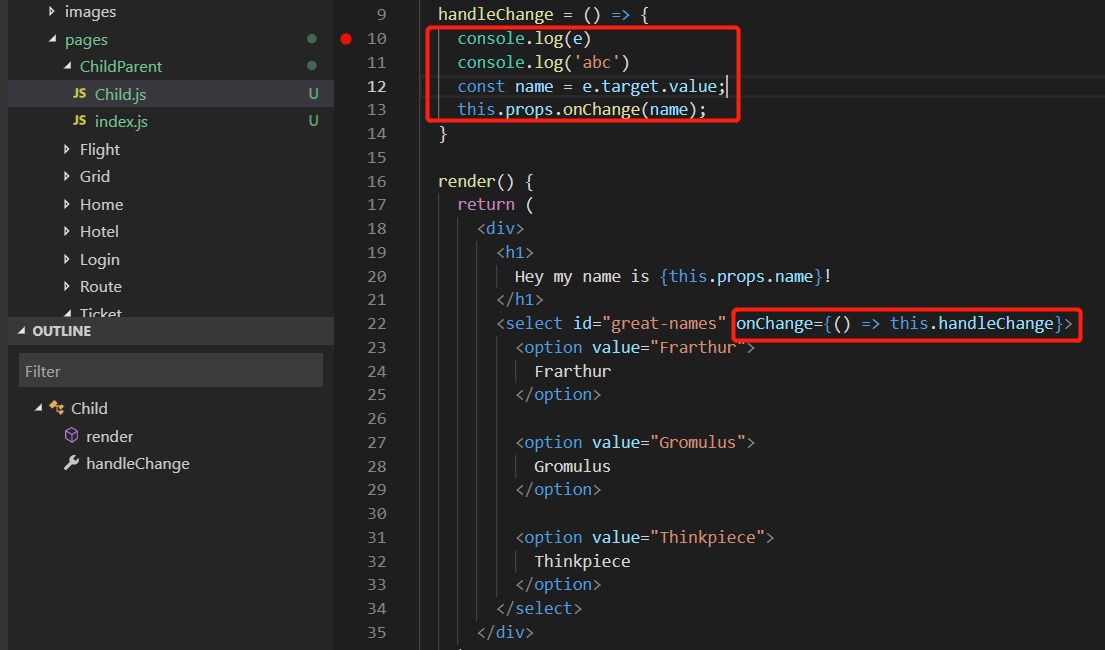
\includegraphics[width=6.5in]{./pics/childUpdateParentsState.png}\\
The body of handleChange won't be executed, don't know why. 当传的是其它参数的时候 (图片中的情形), 在事件触发的地方调用class method需要加(),否则对应的class method的body不会被执行


\subsection{react styles}
在项目中引用某个组件时,如果想对其添加style,则需要将那个组件包裹在div内,接着在div上加style属性,不能直接在那个组件上加style属性 (但是可以找到对应的className在less文件里面加样式)\\
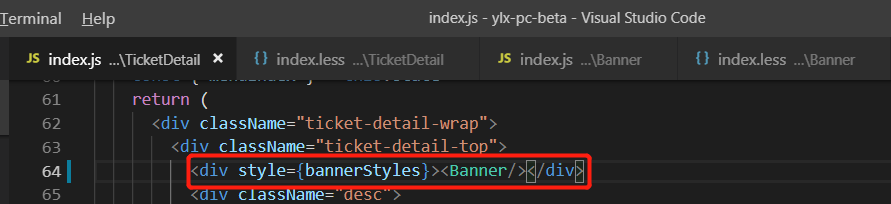
\includegraphics{./pics/styleOnComponent.png}


\subsection{less}
\href{https://medium.com/@joseph0crick/react-css-modules-less-webpack-4-a50d902d0a3}{React + CSS Modules + LESS + Webpack 4}
包含一个完整的less示例

\subsection{Array map method}
\begin{enumerate}
\item 

\item Each child in an array or iterator should have a unique "key" prop

\end{enumerate}

\subsection{react高阶组件 (high order component)}
\begin{itemize}
\item 高阶组件就是接受一个组件作为参数并返回一个新组件的函数

\item 高阶组件是一个函数,并不是组件

\item 尽量使用代理方式的高阶组件

\item 

\end{itemize}



\section{wechat mini program}
\subsection{框架}
\begin{enumerate}

\item 开发者需要做的只是将页面的数据、方法、生命周期函数注册到 框架 中

\item 框架的核心是一个响应的数据绑定系统
\item 整个小程序框架系统分为两部分:视图层(View)和逻辑层(App Service)
\end{enumerate}

\vspace{2in}
小程序~服务号~订阅号~企业号

\section{JavaScript}

\subsection{\href{https://www.cnblogs.com/wangyunhui/p/7511615.html}{js扩展运算符(spread)是三个点(...)}}
作用:将一个数组转为用逗号分隔的参数序列

\subsection{object}
\begin{enumerate}
\item There are only seven fundamental data types in JavaScript, and six of those are the primitive data types: \verb|string, number, boolean, null, undefined|, and \verb|symbol|. With the seventh type, \verb|objects|, we open our code to more complex possibilities

\item Objects are \textit{mutable} meaning we can update them after we create them!

\item You can delete a property from an object with the \verb|delete| operator
\begin{verbatim}
const spaceship = {
  'Fuel Type': 'Turbo Fuel',
  homePlanet: 'Earth',
  mission: 'Explore the universe' 
};

delete spaceship['Fuel Type'];
\end{verbatim}

\item When the data stored on an object is a function we call that a \textit{method}

\item Certain languages have privacy built-in for objects, but JavaScript does not have this feature. Rather, JavaScript developers follow naming conventions that signal to other developers how to interact with a property

\item \verb|typeof()|: in JavaScript, the data type of null is an object. The return value of \verb|typeof()| can be "string" "number" "boolean" "undefined" "object" "function"

\item JavaScript Types are Dynamic:
\begin{verbatim}
var x;           // Now x is undefined
x = 5;           // Now x is a Number
x = "John";      // Now x is a String
\end{verbatim}

\item \textit{avoid} using arrow functions when using \verb|this| in a method

\item Property Value Shorthand:\\
factory function:
\begin{verbatim}
const monsterFactory = (name, age) => {
  return { 
    name: name,
    age: age
  }
};
\end{verbatim}

Imagine if we had to include more properties, that process would quickly become tedious! But we can use a destructuring technique, called \textit{property value shorthand}, to save ourselves some keystrokes
\begin{verbatim}
const monsterFactory = (name, age) => {
  return { 
    name,
    age 
  }
};
\end{verbatim}

\item Destructured Assignment
\begin{verbatim}
const vampire = {
  name: 'Dracula',
  residence: 'Transylvania',
  preferences: {
    day: 'stay inside',
    night: 'satisfy appetite'
  }
};

const { residence } = vampire; 
console.log(residence); // Prints 'Transylvania'
\end{verbatim}
We can even use destructured assignment to grab nested properties of an object:
\begin{verbatim}
const { day } = vampire.preferences; 
console.log(day); // Prints 'stay inside'
\end{verbatim}

\item Built-in Object Methods

object instance methods like: \verb|.hasOwnProperty()|, \verb|.valueOf()|

Object class methods such as \verb|Object.assign()|, \verb|Object.entries()|, and\\ \verb|Object.keys()|

\end{enumerate}

\subsubsection{Looping Through Objects}
JavaScript has given us alternative solution for iterating through objects with the \verb|for...in| syntax




\subsection{class}
\begin{enumerate}

\item Although the subclass automatically inherits the parent methods, you need to use the \verb|super| keyword to set the parent properties

\item static methods: The \verb|.now()| method is static, so you can call it directly from the class, but not from an instance of the class
\begin{verbatim}
static generateName() {
  const names = ['Angel', 'Spike', 'Buffy', 'Willow', 'Tara'];
  const randomNumber = Math.floor(Math.random()*5);
  return names[randomNumber];
}
\end{verbatim}

\item In a \verb|constructor()|, you must always call the \verb|super| method before you can use the \verb|this| keyword — if you do not, JavaScript will throw a reference error, it is best practice to call super on the first line of subclass constructors

\item When multiple classes share properties or methods, they become candidates for \textit{inheritance} — a tool developers use to decrease the amount of code they need to write

\item Notice, we also prepended our property names with underscores (\verb|_name| and \verb|_behavior|), which indicate these properties should not be accessed directly

\end{enumerate}

\subsection{Request}
\begin{enumerate}
\item GET and POST requests can be created a variety of ways
\item Use AJAX to asynchronously request data from APIs. \verb|fetch()| and \verb|async/await| are new functionalities developed in ES6 (promises) and ES8 respectively
\item Promises are a new type of JavaScript object that represent data that will eventually be returned from a request
\item \verb|fetch()| is a web API that can be used to create requests. \verb|fetch()| will return promises
\item We can chain \verb|.then()| methods to handle promises returned by \verb|fetch()|
\item The \verb|.json()| method converts a returned promise to a JSON object
\item \verb|async| is a keyword that is used to create functions that will return promises
\item \verb|await| is a keyword that is used to tell a program to continue moving through the message queue while a promise resolves
\item \verb|await| can only be used within functions declared with \verb|async|
\end{enumerate}

\subsection{Errors}
Errors will prevent a program from executing unless it is handled



\section{CSS}

\subsection{Caveats}
\begin{enumerate}
\item The unit px, if the value is 0 then you can omit the px unit, if it's not 0 then you have to add px

\item 

\end{enumerate}


\subsection{Media Queries}
\begin{itemize}
\item 

\item Rather than set breakpoints based on specific devices (too many different device screen sizes), the best practice is to resize your browser to view where the website naturally breaks based on its content. The dimensions at which the layout breaks or looks odd become your media query breakpoints. Within those breakpoints, we can adjust the CSS to make the page resize and reorganize

\item The points at which media queries are set are called breakpoints. For example, if we want to target tablets that are in landscape orientation, we can create the following breakpoint:
\begin{verbatim}
@media only screen and (min-width: 768px) and (max-width: 1024px) and 
(orientation: landscape) {
    /* CSS ruleset */
}
\end{verbatim}
\verb|and (min-width: 768px)| \textemdash This part of the rule is called a \textit{media feature}, and instructs the CSS compiler to apply the CSS styles to devices with a width of 768px or larger

\end{itemize}

\subsection{CSS Display and Positioning}
\begin{itemize}
\item 即使position设置为absolute,其宽度用百分比表示时是相对于父节点的宽度而言,见\ref{position}

\item Floated elements must have a width specified

\item \verb|Float| works for static and relative positioned elements

\item  If you're simply interested in moving an element as far left or as far right as possible on the page, you can use the \verb|float| property

\end{itemize}	

\subsection{The box model}
\begin{itemize}

\item All major web browsers have a default stylesheet they use in the absence of an external stylesheet. These default stylesheets are known as \textit{user agent stylesheets}. In this case, the term "user agent" is a technical term for the browser

\item The overflow property is set on a parent element to instruct a web browser how to render child elements. For example, if a div's overflow property is set to \verb|scroll|, all children of this div will display overflowing content with a scroll bar.

\item Margin collapse: Unlike horizontal margins, vertical margins do not add. Instead, the larger of the two vertical margins sets the distance between adjacent elements (apply to nested elements as well, maybe there's no nested elements at all {\color{red} I think there is})

ylx-wx-beta
\begin{verbatim}
index.js

import React from 'react'
import './index.less'
import SearchHeader from '../../../components/SearchHeader'

export default class TicketSearch extends React.Component {

	search = (e) => {
		console.log(e.target)
	}
	render() {
		return (
			<div className="hot-search-wrap">
				<SearchHeader showCity={false} onChange={this.search} />
				<div className="content-wrap">
					<div className="head">热门搜索</div>
					<div className="locations">
						<button type="button">武汉花世界·花呆萌乐园</button>
						<button type="button">东湖游船</button>
						<button type="button">光谷步行街</button>
						<button type="button">户部巷</button>
						<button type="button">武汉胜天生态农庄</button>
						<button type="button">姚家山风景区</button>
						<button type="button">武汉东湖风景区</button>
						<button type="button">武汉东湖磨山景区</button>
					</div>

					<div className="history">
						<div className="head">历史搜索</div>
					</div>
				</div>
			</div>
		)
	}
}


index.less

@import '../../../utils/color.less';

.hot-search-wrap {
  .content-wrap {
    margin-top: 70px;
    padding: 0 15px;
    .head {
      margin: 15px 0;
    }
    button {
      display: inline-block;
      padding: 6px;
      border-radius: 5px;
      margin-right: 10px;
      margin-bottom: 6px;
      border: 1px solid blue;
    }
  }
}
\end{verbatim}

\item The \verb|padding| property is often used to expand the background color and make content look less cramped

\item By default, the dimensions of an HTML box are set to hold the raw contents of the box

\end{itemize}


\subsection{Non-Inherited properties}
To name but a few, non-inherited properties are:\\ \verb|width, height, padding, border, margin, position, background|, etc.

\subsection{Learn Responsive Design}
\begin{enumerate}
\item \textbf{Historically}, the em represented the width of a capital letter M in the typeface and size being used. That is no longer the case. Today, the em represents the size of the base font being used. For example, if the base font of a browser is 16 pixels (which is normally the default size of text in a browser), then 1 em is equal to 16 pixels. 2 ems would equal 32 pixels, and so on

\item A high resolution display may have a \verb|min-resolution| of \verb|150dpi|

\item The height property is set to auto, meaning an image's height will automatically scale proportionally with the width

the last line will display images as block level elements (rather than inline-block, their default state)
\begin{verbatim}
.container {
  width: 50%;
  height: 200px;
  overflow: hidden;
}

.container img {
  max-width: 100%;
  height: auto;
  display: block;
}
\end{verbatim}
Images or videos  will shrink to the full width of their container, scale proportionally, and display partially if the image dimensions exceed container dimensions

It's worth memorizing the entire example above. It represents a very common design pattern used to scale images and videos proportionally

\item Percentages are often used to size box-model values, like width and height, padding, border, and margins. They can also be used to set positioning properties (top, bottom, left, right). When percentages are used, elements are sized relative to the dimensions of their parent element (also known as a container) \label{position}\\
\textbf{Note:} Because the box model includes padding, borders, and margins, setting an element's width to 100\% may cause content to overflow its parent container. While tempting, 100\% should only be used when content will not have padding, border, or margin

\item Rem stands for root em. It acts similar to em, but instead of checking parent elements to size font, it checks the root element. The root element is the \verb|<html>| tag

\item \begin{verbatim}
.splash-section {
  font-size: 18px;
}

.splash-section h1 {
  font-size: 1.5em;
}
\end{verbatim}
Instead, a base font size (\verb|18px|) is defined for all text within the \verb|splash-section| element. The second CSS rule will set the font size of all \verb|h1| elements inside of \verb|splash-section| relative to the base font of \verb|splash-section| (18 pixels). The resulting font size of \verb|h1| elements will be 27 pixels.
\end{enumerate}

\subsubsection{Percentages: Padding \& Margin}
\begin{enumerate}
\item When percentages are used to set padding and margin, however, they are calculated based only on the \textit{width} of the parent element.

For example, when a property like \verb|margin-left| is set using a percentage (say \verb|50%|), the element will be moved halfway to the right in the parent container (as opposed to the child element receiving a margin half of its parent's margin)

Vertical padding and margin are also calculated based on the width of the parent

\end{enumerate}

\subsection{display property}
\textbf{Note:} Setting the display property of an element only changes \textbf{how the element is displayed}, NOT what kind of element it is. So, an inline element with \verb|display: block;| is not allowed to have other block elements inside it.

\subsection{Grid layout}
\begin{enumerate}
\item flexbox is really meant for only specific use cases, like navigation bars (navbars)
\end{enumerate}

\subsection{p tag}
\begin{enumerate}
\item \verb|<figcaption><p>The <em>Cosmos</em> is all there is!</p></figcaption>| if you don't add \verb|p| tag then there will be no space before or after \verb|Cosmos|
\end{enumerate}


\section{Node}
Enter repl (read evaluate print loop): type node in command line, exit command \verb|process.exit()|



\section{npm}
\begin{enumerate}

\item 

\item If you're using npm 5, you'll probably also see a package-lock.json file in your directory

\item Useful command \verb|npm show create-react-app version|\\
Get list of locally installed packages: \verb|npm list|, you can find the version of a specific package by passing its name as an argument. For example, \verb|npm list grunt|\\
Get list of globally installed packages: \verb|npm list -g --depth 0|

\item nvm: node version manager, to manage multiple node versions on one operating system

\item To update Node, the most reliable way is to download and install an updated installer package from their website (see link above). To update npm, use the following command in your terminal:
\begin{verbatim}
npm install npm@latest -g
\end{verbatim}
\end{enumerate}

\section{DOM}
\begin{enumerate}

\item \verb|document.createElement()|
\begin{verbatim}
<!DOCTYPE html>
<html>
<head>
  <title>||Working with elements||</title>
</head>
<body>
  <div id="div1">The text above has been created dynamically.</div>
</body>
</html>

document.body.onload = addElement;

function addElement () { 
  // create a new div element 
  var newDiv = document.createElement("div"); 
  // and give it some content 
  var newContent = document.createTextNode("Hi there and greetings!"); 
  // newDiv.textContent = "Hi there and greetings!".
  
  // add the text node to the newly created div
  newDiv.appendChild(newContent);  

  // add the newly created element and its content into the DOM 
  var currentDiv = document.getElementById("div1"); 
  document.body.insertBefore(newDiv, currentDiv); 
}
\end{verbatim}

\item \verb|Document| and \verb|window| objects are the objects whose interfaces you generally use most often in DOM programming. In simple terms, the \verb|window| object represents something like the browser, and the \verb|document| object is the root of the document itself. \verb|Element| inherits from the generic \verb|Node| interface, and together these two interfaces provide many of the methods and properties you use on individual elements

\item That is to say, it's \textit{written} in JavaScript, but it uses the DOM to access the document and its elements
\end{enumerate}


\section{cmd}
\begin{enumerate}

\item 

\item \href{https://stackoverflow.com/questions/41139067/git-log-output-encoding-issues-on-windows-10-command-prompt}{git log output encoding issues on Windows 10 command prompt}

\item Windows clear screen commands:

cls (clear screen) \quad Press Esc key \quad Ctrl + c

\end{enumerate}


\section{中文笔记}
\begin{itemize}

\item 


\item 变量提升:JS会在词法分析阶段,把变量的声明语句提升到作用域的顶部

\end{itemize}


\section{命名规范 Name convention}
\begin{itemize}
\item 线路首页: Route or RouteHome

\item 

\item 

\end{itemize}



\section{Abbr}
\begin{tabular}{ll@{\hspace{3em}}ll@{\hspace{3em}}ll}
% &  &  &  &  &  \\
block & 块级 & inline & 内联 & lexical & 词法作用域 \\
closure & 闭包 & render & 渲染 & container & 容器 \\
content & 内容 & form & 表单 & canvas & 画布 \\
component & 组件 & margin & 外边距 & style & 样式 \\
callback & 回调 & revert & 回滚 & collapse & 折叠 \\
\multicolumn{3}{l}{template string 模板字符串} & \multicolumn{3}{l}{logical operators 逻辑运算符}\\
\multicolumn{3}{l}{object destructure 对象解构}  & \multicolumn{3}{l}{array destructure 数组解构} \\ 
\multicolumn{3}{l}{logical operands: true false}  & \multicolumn{3}{l}{SoC: Separation of Concerns} \\\multicolumn{6}{l}{POSIX: portable operating system interface for unix } \\
\multicolumn{4}{l}{umd: universal module definition} \\
\multicolumn{4}{l}{XSS attack: cross-site scripting attack} \\
\end{tabular}



\end{document}
